\section{Talking to mbed}
\label{sec:talking}

\subsection{Serial Ports}
\label{sub:uart}
\begin{frame}[fragile]
	\frametitle{Serial Ports}
	The Nucleo has one serial port that connects to the computer over USB:
	\begin{lstlisting}[numbers=none]
		Serial pc(USBTX, USBRX);
	\end{lstlisting}
	\vfill
	Every serial port has an associated baud rate (9600, 19200, 115200):
	\begin{lstlisting}[numbers=none]
		pc.baud(int baudrate);
	\end{lstlisting}
	\vfill
	There are methods to test if the port is ready to read or write:
	\begin{lstlisting}[numbers=none,multicols=2]
		pc.readable();
		pc.writeable();
	\end{lstlisting}
	These methods return true if the port is ready.
\end{frame}

\begin{frame}[fragile]
	\frametitle{Reading and Writing Characters}
	The simplest way to talk is a character at a time:
	\begin{lstlisting}[numbers=none,multicols=2]
		char in = pc.getc();
		pc.putc(char out);
	\end{lstlisting}
	To write formatted output:
	\begin{lstlisting}[numbers=none]
		printf(string format (%[flags][width].[precision][key]), ...);
	\end{lstlisting}
	\begin{columns}[T]
		\begin{column}{0.5\textwidth}
			\begin{tabular}{c|l}
				Flag & Description\\
				\hline
				- & Left justify\\
				+ & Force sign character\\
				(space) & Leave a space for sign\\
				0 & Zero padding\\
			\end{tabular}
		\end{column}
		\begin{column}{0.5\textwidth}
			\begin{tabular}{c|l}
				Key & Output\\
				\hline
				d or i & Signed decimal integer\\
				u & Unsigned decimal integer\\
				f & Decimal floating point\\
				e & Scientific notation\\
				c & Character\\
				s & String of characters\\
			\end{tabular}
		\end{column}
	\end{columns}
\end{frame}

\begin{frame}[fragile]
	\frametitle{printf Examples}
	\begin{lstlisting}[caption={Code}]
		printf("Characters: %c %c \n", 'a', 65);
		printf("Decimals: %d %ld\n", 1977, 650000L);
		printf("Preceding with blanks: %10d \n", 1977);
		printf("Preceding with zeros: %010d \n", 1977);
		printf("floats: %4.2f %+.0e %E \n", 3.1416, 3.1416, 3.1416);
		printf("Width trick: %*d \n", 5, 10);
		printf("%s \n", "A string");
	\end{lstlisting}
	\begin{lstlisting}[caption={Output}]
		Characters: a A
		Decimals: 1977 650000
		Preceding with blanks:       1977
		Preceding with zeros: 0000001977
		floats: 3.14 +3e+000 3.141600E+000
		Width trick:    10
		A string
	\end{lstlisting}
\end{frame}

\begin{frame}[fragile]
	\frametitle{Viewing the Serial Port}
	\begin{columns}[T]
		\begin{column}{0.5\textwidth}
			%TODO RealTerm screenshot
			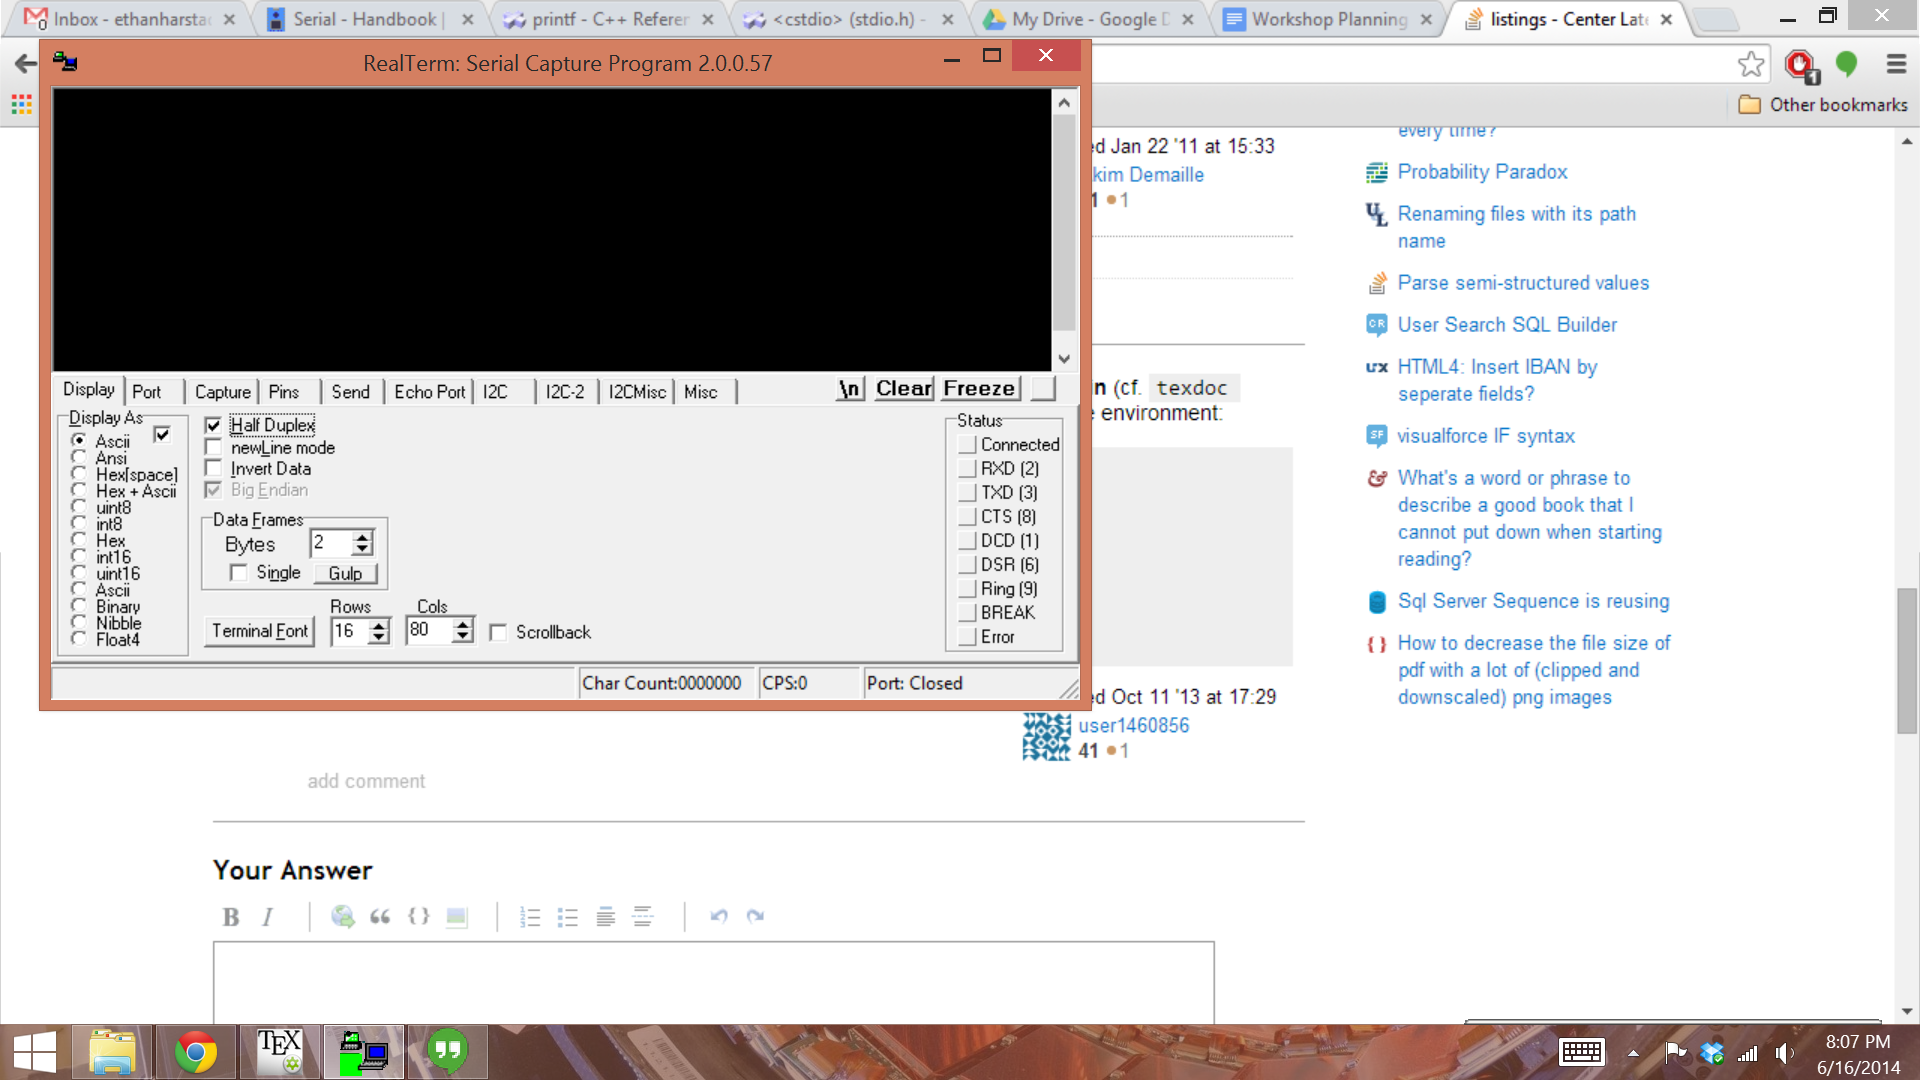
\includegraphics[width=\linewidth]{realterm}
		\end{column}
		\begin{column}{0.5\textwidth}
			\begin{enumerate}
				\item Open RealTerm
				\item Enable "Half Duplex"
				\item Click the "Port" tab
				\item Baud: 9600 and the correct port
				\item Click "Change"
			\end{enumerate}
		\end{column}
	\end{columns}
	\vfill
	Try running a simple sample program:
	\begin{lstlisting}[numbers=none]
		Serial pc(USBTX, USBRX);
		int main() {
		  pc.printf("Hello world!");
		  while(true) {
		    pc.putc(pc.getc() + 1);
		  }
		}
	\end{lstlisting}
\end{frame}

\subsection{Switch/Case Statements}
\label{sub:switch_case}


\subsection{Functions}
\label{sub:functions}


\subsection{For Loops}
\label{sub:for_loops}
